\documentclass[man,12pt,a4paper,floatsintext,draftfirst]{apa6}

% STYLE
% \usepackage{mathptmx} % uses Times font for text and maths

\usepackage{hyperref}
\hypersetup{colorlinks=true,
	linkcolor=blue,
	citecolor=blue,
	urlcolor=blue}

% smaller caption text
\usepackage{caption}
\captionsetup{font=footnotesize}

% MATHS
\usepackage{amsmath}
\usepackage{mathtools} % for \splitfrac
\usepackage{amssymb}

% GRAPHICS
\usepackage{graphicx}
\graphicspath{ {figures/} }     % define relative path to the figures

% CROSS-REFERENCING
% \usepackage{nameref} % for references to sections by name, not number

% REFERENCING
\usepackage{doi}
\usepackage[natbibapa, bibnewpage, doi]{apacite} % use this for APA style




% AUTHOR-DEFINED STUFF
\DeclareMathOperator*{\argmax}{arg\,\!max}

\usepackage{lipsum} % <---------- remove me

\title{My lovely paper}
\shorttitle{Short title of paper here}

\author{Benjamin T. Vincent}
\affiliation{School of Social Sciences, University of Dundee, UK.}

\date{\today}

\begin{document}

\maketitle

\begin{abstract}
 ~This is the abstract \lipsum[1] 
\end{abstract}

\section{Introduction}
This is a reference \citep{Vincent:2015dh}

\lipsum[1-5] % <---------- remove me

\begin{equation}
\label{eq1}
  y = mx+c
\end{equation}

\lipsum[2] % <---------- remove me

\begin{figure}[t!] 
	\centering
	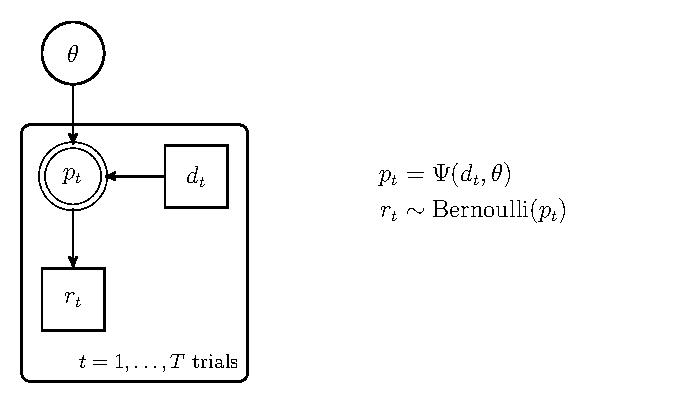
\includegraphics[]{bayes_net_general.pdf} 
	\caption{This is a caption}
	\label{fig:first_figure}
\end{figure}

\lipsum[3] % <---------- remove me

% REFERENCE SECTION
\clearpage
\bibliographystyle{apacite}
\bibliography{my_references}

\end{document}
